\newcommand{\ssat}{\texttt{\#}SAT}
\usetikzlibrary{arrows,positioning}

\subsection{Web Configurators in Action}

\begin{frame}{\myframetitle}
	\begin{mycolumns}[widths={70,30}]
		\myexampletight{Configuring a Notebook}{
			\only<1,3->{\includegraphics[width=\linewidth]{thinkpad-x1-yoga-display}}\only<2|handout:0>{\includegraphics[width=\linewidth]{thinkpad-x1-yoga-display-invalidconf}}
		}
	\mynextcolumn
		\mynote{}{
			can detect mistakes, but provides no explanations or fixes
		}
	\end{mycolumns}
\end{frame}

\begin{frame}{\myframetitle}
	\begin{mycolumns}[widths={70,30}]
		\myexampletight{Still Configuring a Notebook}{
			\includegraphics[width=\linewidth]{thinkpad-x1-yoga-office}
		}
	\mynextcolumn
		\mynote{}{
			allows some feature combinations and not others, prices are opaque
		}
	\end{mycolumns}
\end{frame}

\begin{frame}{\myframetitle}
	\begin{mycolumns}[widths={40,60}]
	\mynextcolumn
		\myexampletight{Configuring a Car}{
			\includegraphics[width=\linewidth]{toyota-aygo-wheels}
		}
	\end{mycolumns}
\end{frame}

\begin{frame}{\myframetitle}
	\begin{mycolumns}[widths={40,60}]
		\mynote{}{
			it is possible to create inconsistent states, leading to an invalid product
		}
	\mynextcolumn
		\myexampletight{Configuring a Car with a Weird Price}{
			\centering\includegraphics[width=.55\linewidth]{toyota-aygo-costs}
		}
	\end{mycolumns}
\end{frame}

\begin{frame}{\myframetitle}
	\begin{mycolumns}[widths={40,60}]
		\mynote{}{
			what happens if we ordered this \ldots?
		}
	\mynextcolumn
		\myexampletight{Configuring a Car with 8 Wheels!}{
			\includegraphics[width=\linewidth]{toyota-aygo-costs3}
		}
	\end{mycolumns}
\end{frame}

\begin{frame}{\myframetitle}
	\begin{mycolumns}[widths={70,30}]
		\myexampletight{Configuring a German Car}{
			\includegraphics[width=\linewidth]{bmw-series1-confassistant-bluetooth}
		}
	\mynextcolumn
		\mynote{}{
			why does the telephone conflict with Microsoft Office?
		}
	\end{mycolumns}
\end{frame}

\subsection{Automated Analysis of Feature Models}

% do everything with one running example (preferably the one from before)
% ie, show an example of an inconsistency and then reveal the issue - can be combined with the MUS explanations

% FM [UVL,attribute,cardinalities,...] -> phi[Prop/FOL/QBF...] -> CNF[BDD/d-DNNF/...] -> SAT[#SAT,AllSat] -> SAT Result -> FM Result
% show this + where it can be varied (BDD, ...) at the end

\begin{frame}{\myframetitle}
	\begin{mycolumns}
		\mynote{Goals}{
			\begin{itemize}
				\item how do such configurators work?
				\item how to avoid inconsistencies?
				\item how to provide explanations and fixes?
    			\item \emph{P2(b)} How to obtain valid configurations automatically?
			\end{itemize}
			$\Rightarrow$ \emph{Automated Analysis of Feature Models}
			% analysis != transformation

			%below: valid cfg = product
		}
	\mynextcolumn
		\myexample{Asking Questions About Feature Models}{
			\begin{itemize}
				\item Is a given configuration valid?
				\item Is there any valid configuration at all?\\
					How many/which valid configurations are there?\\
				\item Is a given feature (de-)selectable at all?\\
					How many/which valid configurations include it?\\
				\item Is a given partial configuration consistent?\\
					How many/which valid configurations include it?\\
				\item \color{gray}{(Which features always occur together?)}
				\item \color{gray}{(Is a given constraint redundant?)}
				\item \color{gray}{(How do two feature model versions differ?)}
				\item \color{gray}{(Why is \ldots? How to fix \ldots?)}
			\end{itemize}
		}
	\end{mycolumns}

	%this section should teach all usual FM/cfg analyses - some in more detail, some only high-level (other SPL analyses come in analyses.tex)

	%list questions we might want to ask a feature model (maybe grouped in the order in which they are discussed)

	%include some simple \#SAT questions (e.g., feature prioritization)

	%how to find out whether a partial configuration is valid? (show decision propagation in FeatureIDE)
\end{frame}

\subsection{SAT, \ssat{}, and AllSAT Solvers}

\begin{frame}{\myframetitle}
	\begin{mycolumns}
		\mydefinition{Recap: Boolean Satisfiability Problem (SAT)}{
			\begin{itemize}
				\item \emph{decision problem}: is there any assignment that satisfies a given formula?
				\item formally: $SAT(\phi) \mequals \exists A \colon \phi(A) = \top$
				\item known to be \emph{NP-complete}:\\
					in theory, difficult to solve if $P \neq NP$;\\
					in practice, solvability depends on domain
				\item answered by \emph{SAT solvers}:\\
					highly-optimized, off-the-shelf tools;\\
					competitively developed over several decades
			\end{itemize}
		}
		\myexample{}{
			\begin{itemize}
				\item $X \pimplies Y$ is satisfiable
				\item $X \por \pnot X$ is satisfiable (even tautological)
				\item $X \pand \pnot X$ is not satisfiable (why?)
			\end{itemize}
		}
	\mynextcolumn
		\mydefinition{Sharp Satisfiability Problem (\ssat{})}{
			\begin{itemize}
				\item \emph{counting problem}: how many assignments satisfy a given formula?
				\item $\ssat(\phi) = \abs{\{A \mid \phi(A) = \top\}}$
				\item known to be \emph{\texttt{\#}P-complete}:\\
					at least as hard as SAT (probably harder)
				\item answered by \emph{\ssat{} solvers}
			\end{itemize}
		}
		\mydefinition{Solution Enumeration Problem (AllSAT)}{
			\begin{itemize}
				\item \emph{enumeration problem}: which assignments satisfy a given formula?
				\item $AllSAT(\phi) = \{A \mid \phi(A) = \top\}$
				\item at least as hard as \ssat{} (probably harder)
				\item answered by \emph{AllSAT solvers}
			\end{itemize}
		}
	\end{mycolumns}
\end{frame}

\subsection{Solver-Based Analysis of Feature Models}

\begin{frame}{\myframetitle}
	\begin{mycolumns}
		\myexample{Asking Questions About Feature Models}{
			\begin{itemize}
				\item Is a given configuration valid? $\Rightarrow$ \emph{evaluate}
				\item \emph{Is} there any valid configuration at all?\\
					\emph{How many}/\emph{which} valid configurations are there?\\
				\item \emph{Is} a given feature (de-)selectable at all?\\
					\emph{How many}/\emph{which} valid configurations include it?\\
				\item \emph{Is} a given partial configuration consistent?\\
					\emph{How many}/\emph{which} valid configurations include it?\\
			\end{itemize}
		}
		\mynote{Choosing the Right Solver Class}{
			\begin{itemize}
				\item ``is''~~~~~~~~~~~~$\approx$ SAT solver query
				\item ``how many''~$\approx$ \ssat{} solver query
				\item ``which''~~~~~~\,$\approx$ AllSAT solver query
			\end{itemize}
		}
	\mynextcolumn
		\mydefinition{Feature-Model Analysis Process}{
			\centering
			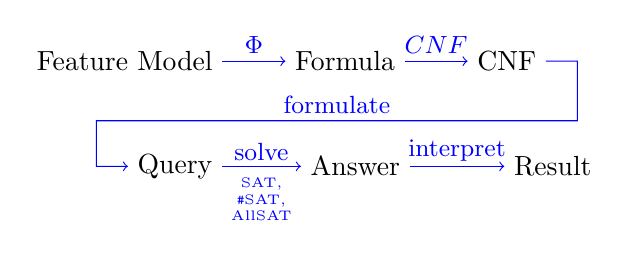
\begin{tikzpicture}
				\tikzset{block/.style={align=center,minimum height=5mm}}
				\node [block] (fm) {Feature Model};
				\node [block, right =8mm of fm] (formula) {Formula};
				\node [block, right =8mm of formula] (cnf) {CNF};
				\node [block, below right =8mm and -12mm of fm] (query) {Query};
				\node [block, right =10mm of query] (answer) {Answer};
				\node [block, right =12mm of answer] (result) {Result};
				\node [coordinate, below right =5mm and 4mm of cnf] (right) {};
				\node [coordinate, above left =3mm and 4mm of query] (left) {};
				\path[draw,->,color=blue] (fm) edge node[yshift=2mm] {\small $\Phi$} (formula)
							(formula) edge node[yshift=2mm] {\small $CNF$} (cnf)
							(cnf.east) -| (right) -- node[yshift=2mm] {\small formulate} (left) |- (query)
							(query) edge node[yshift=-2mm] {\small \parbox{10mm}{\centering solve\\[1ex]\tiny SAT,\\\ssat{},\\AllSAT}} (answer)
							(answer) edge node [yshift=2mm]{\small interpret} (result);
			\end{tikzpicture}
		}
		%below we assume phi to be in cnf
	\end{mycolumns}
\end{frame}

%sat, taut
%	extensions to SAT solver interface (harder to implement):
%	when SAT = true, some give a satisfying assignment (for optimizations)
%	wen SAT = false, some give a MUS (for explanations) % see master theses of T. Günther, S. Ananieva

\subsection{Consistency and Cardinality of Feature Models}

\begin{frame}{\myframetitle}
	\begin{mycolumns}[t]
		\emph{Consistency of Feature Models (SAT)}
		\mydefinition{Void/Consistent Feature Model}{
			\begin{itemize}
				\item are there grave modeling errors?
				\item is it possible to configure any product at all?
			\end{itemize}
			\centering
			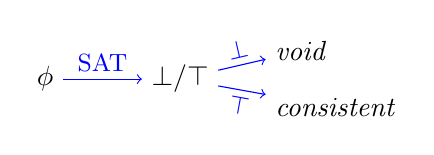
\begin{tikzpicture}
				\tikzset{block/.style={align=center,minimum height=5mm}}
				\node [block] (query) {$\phi$};
				\node [block, right =10mm of query] (answer) {$\bot/\top$};
				\node [block, above right =-2mm and 6mm of answer] (void) {\emph{void}};
				\node [block, below right =-2mm and 6mm of answer] (notvoid) {\emph{consistent}};
				\path[draw,->,color=blue] (query) edge node[yshift=2mm] {\small SAT} (answer)
							(answer) edge node [yshift=2mm,sloped]{\small $\bot$} (void)
							(answer) edge node [yshift=-2mm,sloped]{\small $\top$} (notvoid);
			\end{tikzpicture}
		}
		\mynextcolumn
		\emph{Cardinality of Feature Models (\ssat{})}
		\mydefinition{How many products are there?}{
			\centering
			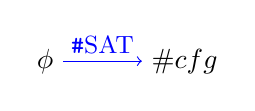
\begin{tikzpicture}
				\tikzset{block/.style={align=center,minimum height=5mm}}
				\node [block] (query) {$\phi$};
				\node [block, right =10mm of query] (answer) {$\#cfg$};
				\path[draw,->,color=blue] (query) edge node[yshift=2mm] {\small \ssat{}} (answer);
			\end{tikzpicture}
		}
		\mydefinition{Variability Factor: Share of Products?}{
			\centering
			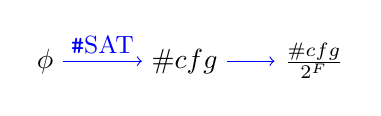
\begin{tikzpicture}
				\tikzset{block/.style={align=center,minimum height=5mm}}
				\node [block] (query) {$\phi$};
				\node [block, right =10mm of query] (answer) {$\#cfg$};
				\node [block, right =6mm of answer] (num) {$\frac{\#cfg}{2^{\abs{F}}}$};
				\path[draw,->,color=blue] (query) edge node[yshift=2mm] {\small \ssat{}} (answer)
							(answer) edge node [yshift=2mm,sloped]{} (num);
			\end{tikzpicture}
		}
	\end{mycolumns}
	\begin{mycolumns}[t]
		\myexampletight{}{
			\leftandright{
				\centering
				{\small\featureDiagram{Root,abstract[X,concrete,alternative][Y,concrete]}\\$\pnot (X \por Y)$}

				void
			}{
				\centering
				{\small\featureDiagram{Root,abstract[X,concrete,alternative][Y,concrete]}\\$X \por Y$}

				consistent
			}
		}
		\mynextcolumn
		\myexampletight{}{
			\leftandright{
				\centering
				{\small\featureDiagram{Root,abstract[X,concrete,alternative][Y,concrete]}\\$\pnot (X \por Y)$}

				$0$ products, VF $0$
			}{
				\centering
				{\small\featureDiagram{Root,abstract[X,concrete,alternative][Y,concrete]}\\$X \por Y$}

				$2$ products, VF $\frac{2}{8}$
			}
		}
	\end{mycolumns}
	%for each analysis, also list \#SAT encoding
	%to WHICH DEGREE is a FM consistent (i.e., degree of freedom / variability factor)?

	%also list explanations / MUS (very shortly)
\end{frame}

\begin{frame}{\myframetitle}
	\begin{mycolumns}[t]
		\emph{Enumeration of Feature Models (AllSAT)}
		\mydefinition{All Products}{
			\begin{itemize}
				\item recall \emph{P2(b)}: How to obtain valid configurations automatically?
			\end{itemize}
			\centering
			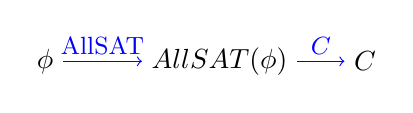
\begin{tikzpicture}
				\tikzset{block/.style={align=center,minimum height=5mm}}
				\node [block] (query) {$\phi$};
				\node [block, right =10mm of query] (answer) {$AllSAT(\phi)$};
				\node [block, right =6mm of answer] (num) {$C$};
				\path[draw,->,color=blue] (query) edge node[yshift=2mm] {\small AllSAT} (answer)
							(answer) edge node [yshift=2mm,sloped]{\small $C$} (num);
			\end{tikzpicture}
		}
		\myexampletight{}{
			\leftandright{
				\centering
				{\small\featureDiagram{Root,abstract[X,concrete,alternative][Y,concrete]}\\$\pnot (X \por Y)$}

				$\varnothing$
			}{
				\centering
				{\small\featureDiagram{Root,abstract[X,concrete,alternative][Y,concrete]}\\$X \por Y$}

				$\{\{Root, X\},\{Root, Y\}\}$
			}
		}
		\mynextcolumn
		% representations slide?
	\end{mycolumns}
\end{frame}

\subsection{Core and Dead Features} % + these are variability smells
\begin{frame}{\myframetitle}
	can a feature be chosen at all? is it false-optional?
	to WHICH DEGREE is a feature core/dead? feature prioritization

	f core iff $SAT(\phi and not f) = \bot$
	
	f dead iff $SAT(\phi and f) = \bot$

	applications: find anomalies/inconsistencies (false-optional), commonality, feature prioritization
\end{frame}

\subsection{Partial Configurations}
\begin{frame}{\myframetitle}
	can a partial configuration be completed?
	can also be connected to Chico's \#SAT applications

	note that this is a generalization of void/core/dead

	total configurations were defined before, now expand this definition to a tuple $(sel, desel)$ and explain why

	applications: ...
\end{frame}

\subsection{Redundant Constraints (?)}
\begin{frame}{\myframetitle}
	... % include this? it has no real #SAT equivalent
\end{frame}

\subsection{Other Analyses}
\begin{frame}{\myframetitle}
	list some more analyses/questions

	atomic sets, determinate features

	probably too much:
	FM edits?
	redundant constraints?

	%explanations?
\end{frame}

% maybe combine Challenges/Experiences? or flip them?
\subsection{Challenges}
\begin{frame}{\myframetitle}
	how is SAT (before: a black box) implemented (very broadly)?

	solvers have parameters, heuristics (variable ordering/assignment, restarts, ...)

	there are SAT solvers that do not use CNF, there are other techniques entirely (BDD, d-DNNF)

	CNF/DIMACS transformation

	non-Boolean requires richer theories (SMT, CSP)
\end{frame}

\subsection{Experiences} % performance / efficiency
\begin{frame}{\myframetitle}
	show a few diagrams with performance on large models

	(may even be implemented concretely as BDD)

	only with Boolean formulas can we get really performant results today

	BDDs are hard to build, but have large payoff (maybe one slide on the abstract concept of knowledge compilation, without too many details?)

	most of this is implemented in FeatureIDE, the configurator is a clever combination of the techniques explained above (Boolean constraint/decision propagation) % show linux configurator

		%at the end (what else is there?): in practice, we also have non-Boolean features/attributes/constraints over attributes (more details on efficiency in third block)

	%there is evidence (Knueppel) that the full expressive power of Boolean formulas is needed for real-world formulas

\end{frame}

% end goal: the lecture shows how to realize a automated configurator that does not allow invalid configurations

\subsection{Challenges of Feature Modeling}

\begin{frame}{\myframetitle}
	scoping: which features do we want to deliver? (vl 8,12)

	interactions: which dependencies between feature are there? (vl 9)

	new tools, languages, experts/consultants, ...
\end{frame}

% later on allsat: DNF as opposition? subtractive/additive definition?

% describe sat, #sat, allsat
% describe size of product lines (chico)

% \myexampletight{Industrial Configuration Spaces \mysource{\evaluatingsharpsatsolvers}}{
% 	\centering\evaluatingsharpsatsolverslink{\includegraphics[width=\linewidth,page=6,trim=50 210 320 440,clip]{2020/2020-VaMoS-Sundermann}}
% }